\documentclass[serif]{beamer}\usepackage[]{graphicx}\usepackage[]{color}
%% maxwidth is the original width if it is less than linewidth
%% otherwise use linewidth (to make sure the graphics do not exceed the margin)
\makeatletter
\def\maxwidth{ %
  \ifdim\Gin@nat@width>\linewidth
    \linewidth
  \else
    \Gin@nat@width
  \fi
}
\makeatother

\definecolor{fgcolor}{rgb}{0.345, 0.345, 0.345}
\newcommand{\hlnum}[1]{\textcolor[rgb]{0.686,0.059,0.569}{#1}}%
\newcommand{\hlstr}[1]{\textcolor[rgb]{0.192,0.494,0.8}{#1}}%
\newcommand{\hlcom}[1]{\textcolor[rgb]{0.678,0.584,0.686}{\textit{#1}}}%
\newcommand{\hlopt}[1]{\textcolor[rgb]{0,0,0}{#1}}%
\newcommand{\hlstd}[1]{\textcolor[rgb]{0.345,0.345,0.345}{#1}}%
\newcommand{\hlkwa}[1]{\textcolor[rgb]{0.161,0.373,0.58}{\textbf{#1}}}%
\newcommand{\hlkwb}[1]{\textcolor[rgb]{0.69,0.353,0.396}{#1}}%
\newcommand{\hlkwc}[1]{\textcolor[rgb]{0.333,0.667,0.333}{#1}}%
\newcommand{\hlkwd}[1]{\textcolor[rgb]{0.737,0.353,0.396}{\textbf{#1}}}%

\usepackage{framed}
\makeatletter
\newenvironment{kframe}{%
 \def\at@end@of@kframe{}%
 \ifinner\ifhmode%
  \def\at@end@of@kframe{\end{minipage}}%
  \begin{minipage}{\columnwidth}%
 \fi\fi%
 \def\FrameCommand##1{\hskip\@totalleftmargin \hskip-\fboxsep
 \colorbox{shadecolor}{##1}\hskip-\fboxsep
     % There is no \\@totalrightmargin, so:
     \hskip-\linewidth \hskip-\@totalleftmargin \hskip\columnwidth}%
 \MakeFramed {\advance\hsize-\width
   \@totalleftmargin\z@ \linewidth\hsize
   \@setminipage}}%
 {\par\unskip\endMakeFramed%
 \at@end@of@kframe}
\makeatother

\definecolor{shadecolor}{rgb}{.97, .97, .97}
\definecolor{messagecolor}{rgb}{0, 0, 0}
\definecolor{warningcolor}{rgb}{1, 0, 1}
\definecolor{errorcolor}{rgb}{1, 0, 0}
\newenvironment{knitrout}{}{} % an empty environment to be redefined in TeX

\usepackage{alltt}
\usetheme{Boadilla}
\usepackage{graphicx}
\usepackage[draft]{animate}
\usepackage{breqn}
\usepackage{xcolor}
\usepackage{booktabs}
\usepackage{tikz}
\usetikzlibrary{decorations.pathreplacing}
\usetikzlibrary{shapes,arrows,positioning,shadows}
\usepackage{subfig}
\usepackage{pgf}

% change format of enumerated lists
\setbeamertemplate{enumerate items}[default]
\setbeamertemplate{navigation symbols}{}

% macros
\newcommand{\emtxt}[1]{\textbf{\textit{#1}}}

% tikz objects
\tikzstyle{decision} = [diamond, draw, text width=6em, text badly centered, inner sep=2pt, top color=white, bottom color=cavalcanti3]
\tikzstyle{block} = [rectangle, draw, text width=10em, text centered, rounded corners, minimum height=3em, minimum width=8em, top color = white, bottom color=cavalcanti3]
\tikzstyle{declare} = [rectangle, draw, text width=10em, text centered, minimum height=3em, minimum width=8em, top color = white, bottom color=cavalcanti3]

% knitr setup


% dependent data


% custom colors
\definecolor{cavalcanti1}{HTML}{D8B70A}\definecolor{cavalcanti2}{HTML}{02401B}\definecolor{cavalcanti3}{HTML}{A2A475}\definecolor{cavalcanti4}{HTML}{81A88D}\definecolor{cavalcanti5}{HTML}{972D15}

% my custom ggplot theme


% figure used on title page


\setbeamercolor{title}{fg=cavalcanti5} % main title
\setbeamercolor{frametitle}{fg=cavalcanti2, bg=cavalcanti3} % frame titles
\setbeamercolor{structure}{fg=cavalcanti4} % bottom banner
\setbeamercolor{normal text}{fg=cavalcanti5}
\usebackgroundtemplate{
\includegraphics[height=\paperheight,width=\paperwidth]{fig/back_tmp.pdf}}
\IfFileExists{upquote.sty}{\usepackage{upquote}}{}
\begin{document}

\title[Evaluating Trends in Gulf Estuaries]{\textbf{A Novel Approach for Evaluation of Water Quality Trends in Gulf Coast Estuaries}}
\author[Beck, Hagy, Murrell]{Marcus W. Beck\inst{1} \and James D. Hagy III\inst{2} \and Michael C. Murrell\inst{2}}

\institute[EPA]{\inst{1} ORISE post-doc, USEPA National Health and Environmental Effects Research Laboratory, Gulf Ecology Division, \href{mailto:beck.marcus@epa.gov}{beck.marcus@epa.gov} \and \inst{2} USEPA National Health and Environmental Effects Research Laboratory, Gulf Ecology Division}

\date{Dec. 3, 2014}

\titlegraphic{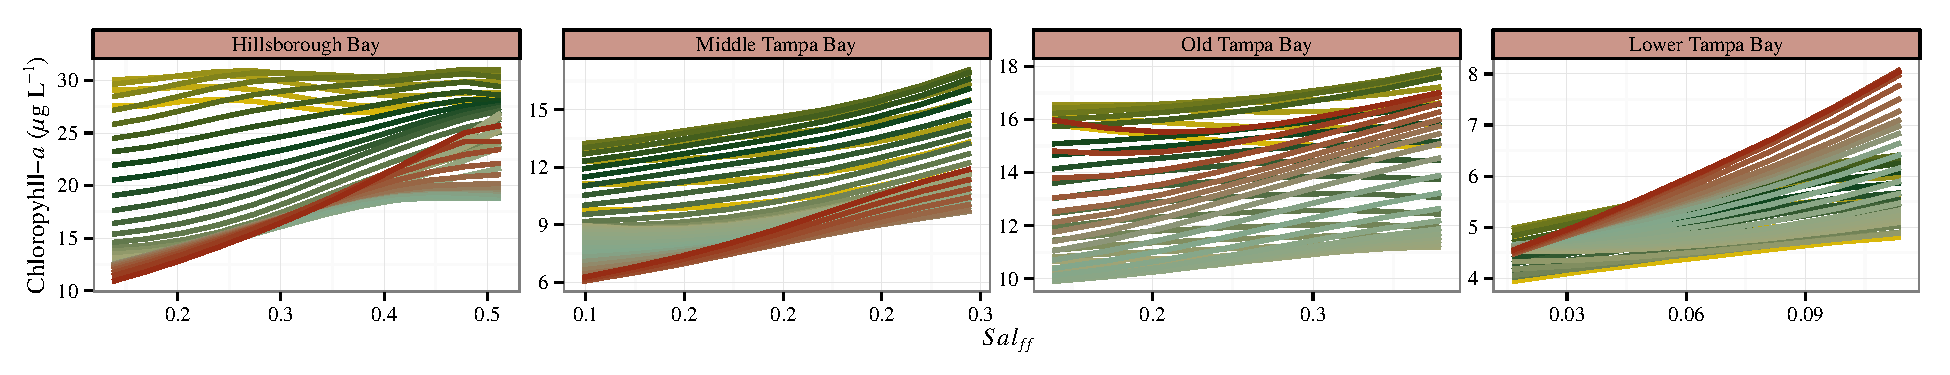
\includegraphics[width=0.9\linewidth]{fig/title_plo.pdf}}

%%%%%%
\begin{frame}[shrink]
\titlepage
\end{frame}

\section{Background}

%%%%%%
\begin{frame}{\textbf{Managing coastal waters}}{\textbf{How do we use data?}}
The foundation of most management programs is a strong monitoring network \\~\\
Monitoring provides information for decision-making based on apparent trends...
\vspace{0.2in}
\begin{center}
\emtxt{What are the changes in water quality over time?}\\~\\
\emtxt{Are these changes `good' or `bad' based on our management objectives?}\\~\\
\emtxt{What may have caused these changes?}
\end{center}
\end{frame}

%%%%%%
\begin{frame}{\textbf{Managing coastal waters}}{\textbf{How do we use data?}}
\emtxt{The good news}: We are getting better at monitoring - standardized, automated, increased coverage, real-time/continuous \\~\\
\emtxt{The bad news}: Our ability to use these data for decision-making has not kept pace with availability! \\~\\


{\centering 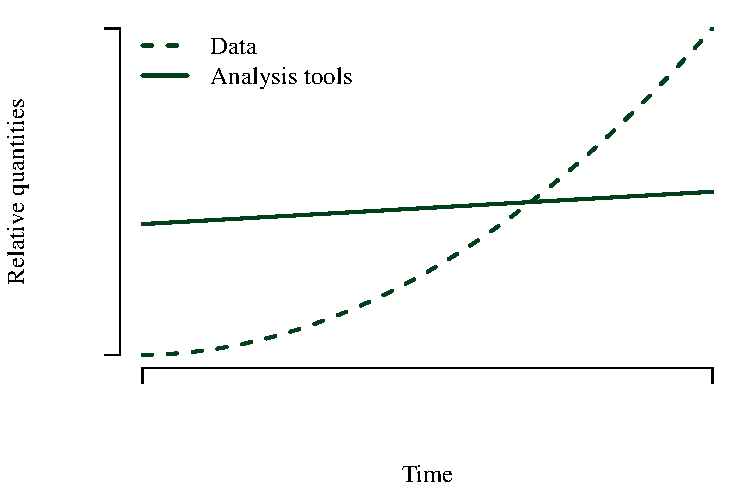
\includegraphics[width=0.55\textwidth]{fig/theo} 

}



\end{frame}

%%%%%%
\begin{frame}{\textbf{Managing coastal waters}}{\textbf{How do we use data?}}
We have the data but often lack appropriate tools to unambiguously and quantitatively characterize trends \\~\\
\emtxt{Challenge 1:} We must first define  `trend' - what does this mean in the context of our management objectives? \\~\\
\emtxt{Challenge 2:} We must use tools that can leverage the descriptive capabilities of large datasets \\~\\
Our research explores novel techniques to address these challenges:\\~\\
\emtxt{Case 1:} Chlorophyll drivers in Tampa Bay \\~\\
\emtxt{Case 2:} Improving estimates of ecosystem metabolism 
\end{frame}

\section{Case 1: Tampa Bay}

% tampa bay map, w/ inset


%%%%%%
\begin{frame}{\textbf{Case 1: Tampa Bay}}{\textbf{Describing drivers of chlorophyll}}
\begin{columns}
\begin{column}{0.5\textwidth}
\begin{itemize}
\item Four bay segments\\~\\
\item Monthly wq data at 50 stations from 1974 to present \\~\\
\item Longitudinal profile of nutrient load and salinity \\~\\
\end{itemize}
\vspace{0cm}\hspace*{15pt}\scalebox{0.7}{\hbox{\tiny Data from \cite{TBEP11}}}
\end{column}
\begin{column}{0.5\textwidth}
\centerline{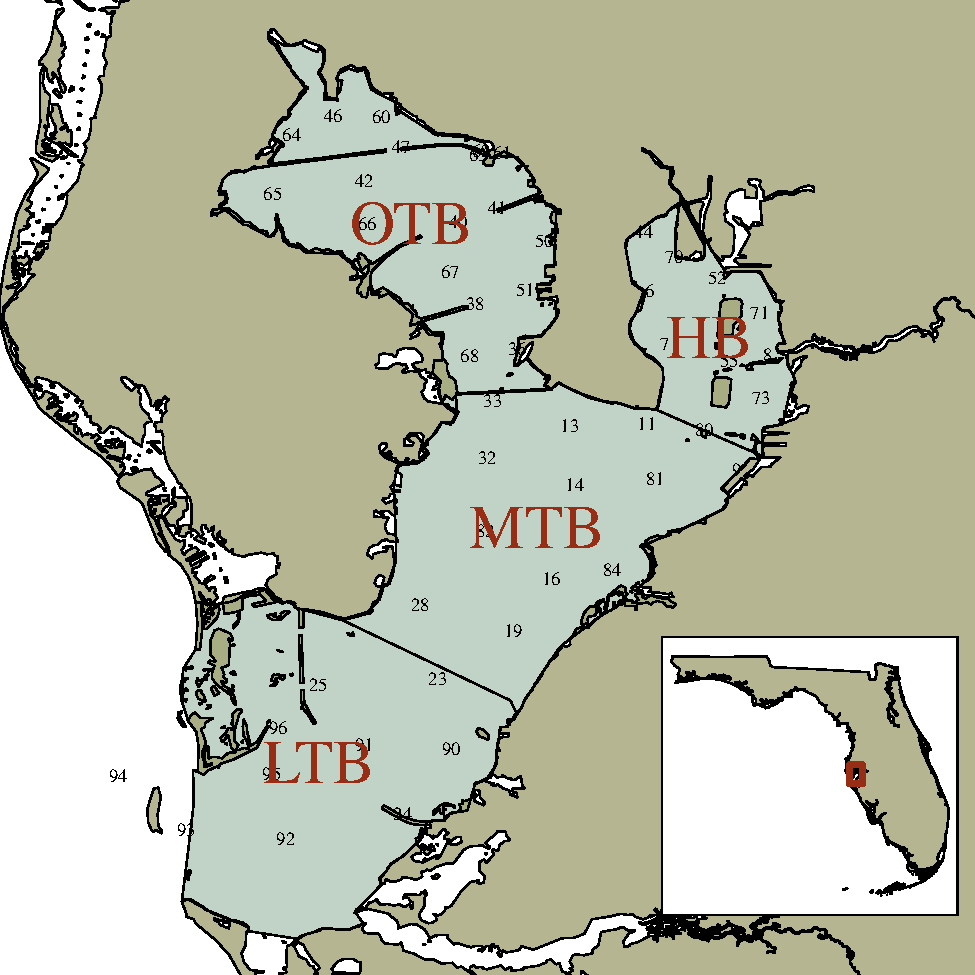
\includegraphics[width = \textwidth]{fig/tb_map.pdf}}
\end{column}
\end{columns}
\end{frame}

%%%%%%
\begin{frame}{\textbf{Case 1: Tampa Bay}}{\textbf{Describing drivers of chlorophyll}}
\begin{figure}[!ht]


{\centering 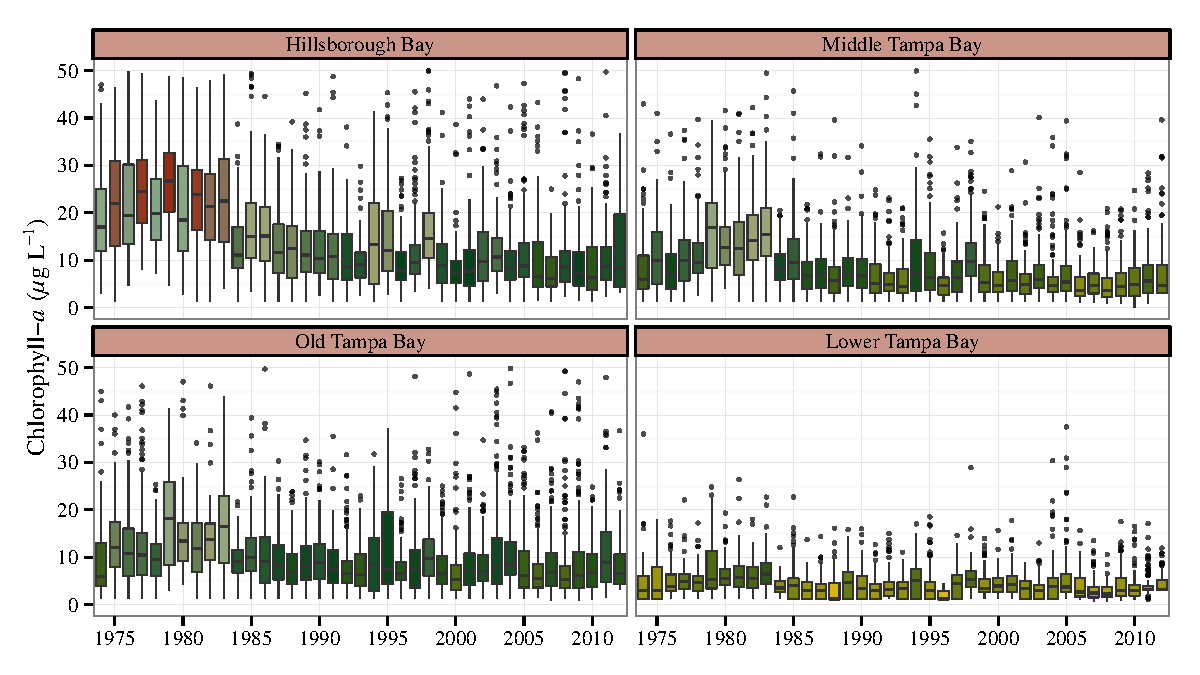
\includegraphics[width=\linewidth]{fig/annual_chl} 

}

\caption[Annual trends in chlorophyll for each bay segment]{Annual trends in chlorophyll for each bay segment.\label{fig:annual_chl}}
\end{figure}


\end{frame}

% variation in chl by year, season, and management

%%%%%%
\begin{frame}{\textbf{Case 1: Tampa Bay}}{\textbf{Describing drivers of chlorophyll}}
What affects our interpretation of chlorophyll response to nutrients?
\vspace{-0.1in}
\captionsetup[subfloat]{captionskip=0pt, position=top}
\begin{figure}
\centering
\subfloat[]{
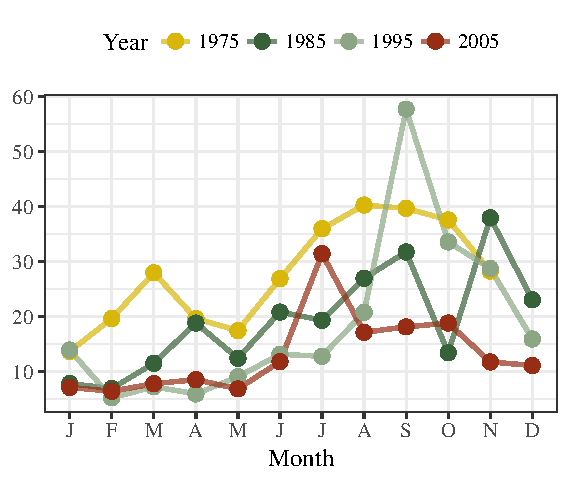
\includegraphics[width=0.46\textwidth,page=1,trim=0.2in 0in 0in 0.35in,clip]{fig/salmoyr.pdf}
\label{fig:salmoyr1}
}
\subfloat[]{
\includegraphics[width=0.46\textwidth,page=2,trim=0.2in 0in 0in 0.35in,clip]{fig/salmoyr.pdf}
\label{fig:salmoyr2}
}

\leavevmode\smash{\makebox[0pt]{\hspace{0em}% HORIZONTAL POSITION           
  \rotatebox[origin=l]{90}{\hspace{3em}% VERTICAL POSITION
    {\color{black} Chlorophyll-\textit{a}}}}}
    \hspace{0pt plus 1filll}\null

\caption{Variation in chlorophyll by {\color{cavalcanti5}\protect\subref{fig:salmoyr1}} time and {\color{cavalcanti5}\protect\subref{fig:salmoyr2}} salinity and management in Hillsborough Bay.  Panel {\color{cavalcanti5}\protect\subref{fig:salmoyr1}} is colored before and after wastewater treatment in 1979.}
\label{fig:salmoyr}
\end{figure}
\captionsetup[subfloat]{position=top}
\end{frame}

%%%%%%
\begin{frame}{\textbf{Case 1: Tampa Bay}}{\textbf{Describing drivers of chlorophyll}}
Given the observed changes over time and the available data -- Can we... 
\begin{itemize}
\item ...provide a natural history of water quality that is temporally consistent with drivers of change (i.e., context for trend evaluation)?
\item ...characterize changes in extreme events in addition to describing the mean response?  
\item ...improve our understanding of the nutrient-response paradigm in estuaries?
\end{itemize}
\end{frame}

%%%%%%
\begin{frame}{\textbf{Case 1: Tampa Bay}}{\textbf{Describing drivers of chlorophyll}}
The \emtxt{weighted regression (WRTDS)} model is being developed by USGS for pollutant modelling in rivers \cite{Hirsch10}\\~\\
Based on the idea that pollution concentration is a function of \emtxt{time}, \emtxt{discharge}, and \emtxt{season}\\~\\
\emtxt{Problem:} We want to see if management has an effect on reducing pollutant load over time, but pollutant load varies with discharge.\\~\\
\emtxt{Solution:} Develop a model that accounts for changes in relationships between drivers of pollution over time.\\~\\
\emtxt{Adaptation:} Can this approach be used to evaluate chlorophyll trends in Tampa Bay?
\end{frame}



%%%%%%
\begin{frame}{\textbf{Case 1: Tampa Bay}}{\textbf{Describing drivers of chlorophyll}}
How does weighted regression work?
\begin{center}
\animategraphics[controls,width=\linewidth]{12}{fig/wtex}{}{} %frame rate is 12 per/sec
\end{center}
\end{frame}



%%%%%%
\begin{frame}{\textbf{Case 1: Tampa Bay}}{\textbf{Describing drivers of chlorophyll}}
Results can also be normalized by predictors -- salinity
\begin{figure}
\centerline{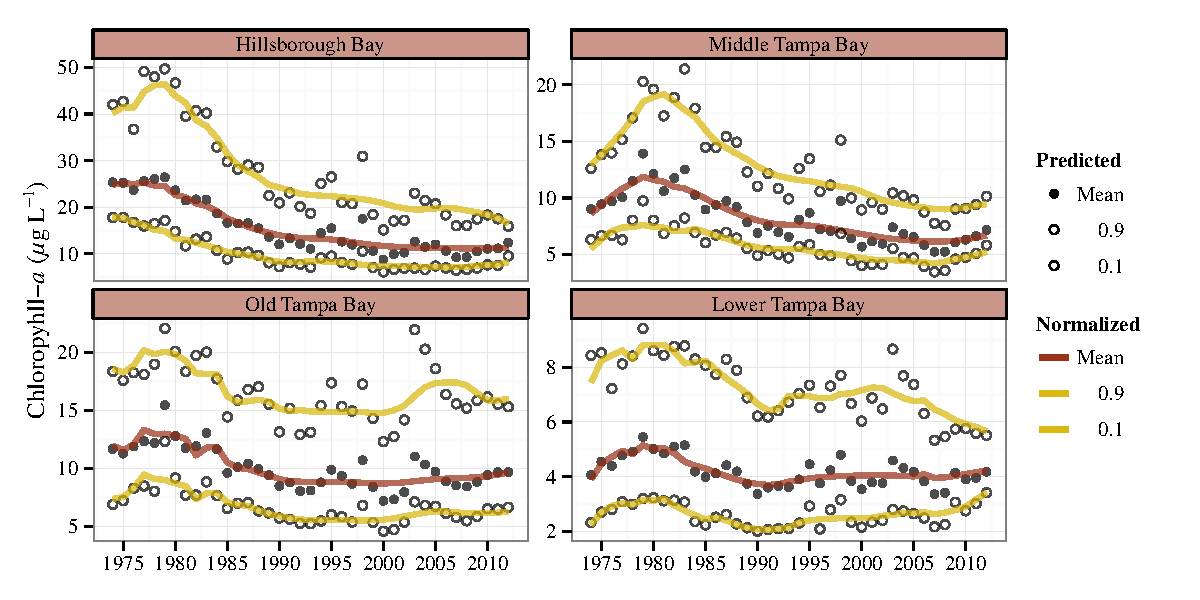
\includegraphics[width = \textwidth]{fig/prdnrm.pdf}}
\caption{Predicted and salinity-normalized annual chlorophyll by segment.}
\end{figure}
\end{frame}



%%%%%%
\begin{frame}{\textbf{Case 1: Tampa Bay}}{\textbf{Describing drivers of chlorophyll}}
Because the model is dynamic, we have parameters describing the relationship of chlorophyll with other factors specific to different time periods \\~\\
\begin{columns}[T]
\begin{column}{0.45\textwidth}
\centerline{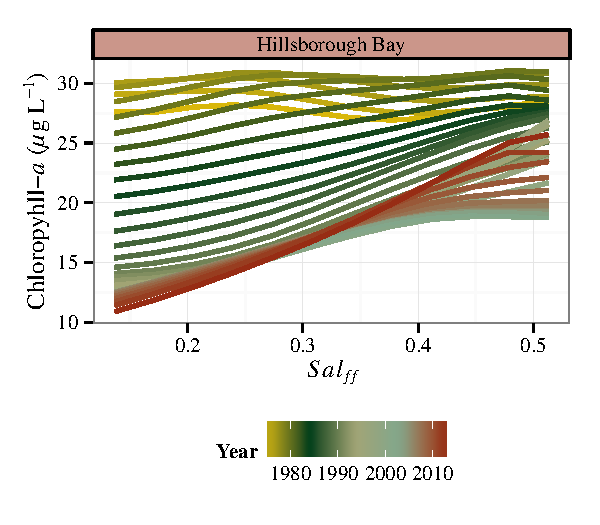
\includegraphics[width = \textwidth]{fig/hill.pdf}}
\end{column}
\begin{column}{0.45\textwidth}
\begin{itemize}
\item Early period (blue) - point-sources
\item Late period (red) - non-point sources
\item Chlorophyll shows increasing response to freshwater input in recent years
\end{itemize}
\end{column}
\end{columns}
\end{frame}

% figure used on title page


%%%%%%
\begin{frame}{\textbf{Case 1: Tampa Bay}}{\textbf{Describing drivers of chlorophyll}}
What does this mean for Tampa Bay and other Gulf Coast estuaries?\\~\\
\begin{itemize}
\item Predictions followed observed chlorophyll -- but increased clarity in the description
\item More detailed evaluation of trends allows greater insight into drivers of change\\~\\
\end{itemize}
The model parameters show us a picture...
\centerline{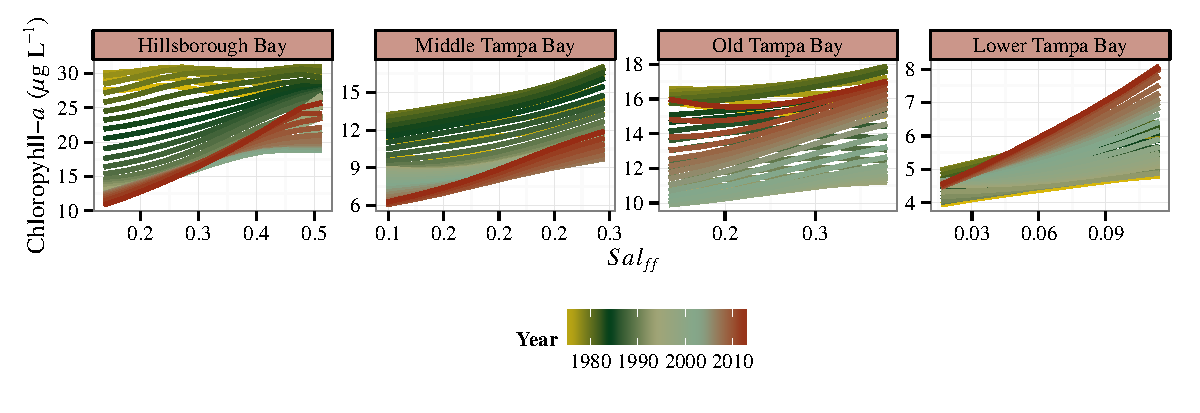
\includegraphics[width = 0.9\textwidth]{fig/title_plo2.pdf}}
\end{frame}

\section{Case 2: Improving metabolism estimates}

%%%%%%
\begin{frame}{\textbf{Case 2: Improving estimates of metabolism}}{\textbf{Application to Gulf Coast estuaries}}
The `Odum' open-water method has been used for decades to estimate rates of ecosystem metabolism \scriptsize \cite{Odum56} \\~\\
\normalsize
\begin{center}
$\frac{\delta DO}{\delta t} = P - R + D$
\end{center}
Metabolic rates provide a measure of productivity in a system - are estuaries sources or sinks of organic matter? \scriptsize \cite{Caffrey14}
\normalsize \\~\\
Applications to estuarine monitoring data have been somewhat successful - why?? 
\end{frame}

%%%%%%
\begin{frame}{\textbf{Case 2: Improving estimates of metabolism}}{\textbf{Application to Gulf Coast estuaries}}
The `Odum' method assumes DO represents biological processes...


{\centering 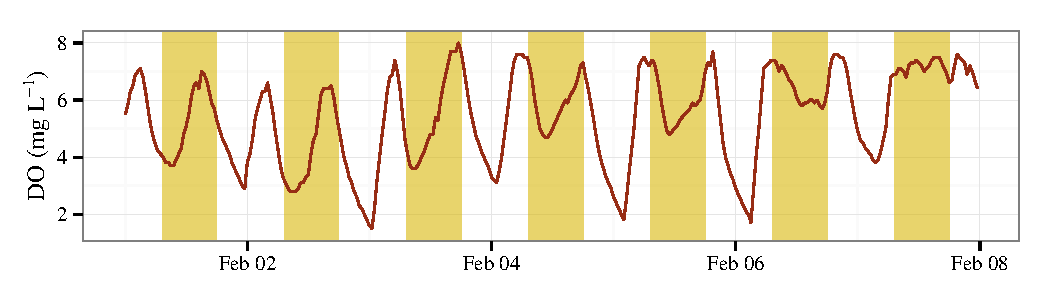
\includegraphics[width=0.95\textwidth]{fig/sapdo} 

}





{\centering 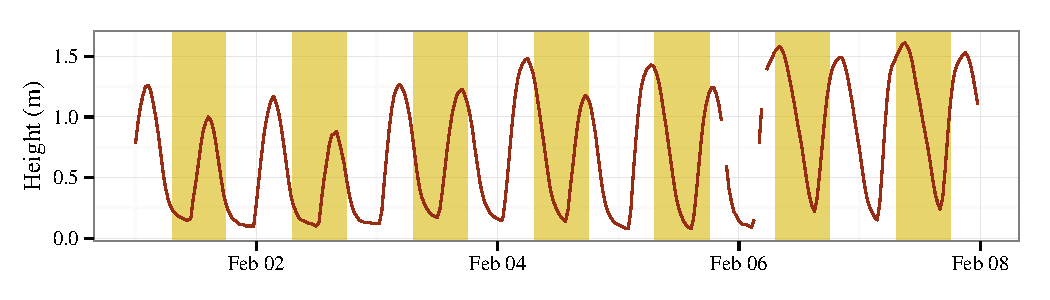
\includegraphics[width=0.95\textwidth]{fig/saptide} 

}



\end{frame}

%%%%%%
\begin{frame}{\textbf{Case 2: Improving estimates of metabolism}}{\textbf{Application to Gulf Coast estuaries}}
\emtxt{Challenge 1:} We want to provide an accurate estimate of metabolism using DO time series to evaluate trends over time \\~\\
\emtxt{Challenge 2:} DO time series may represent variation from physical and biological processes \\~\\
The weighted regression approach could be used here...
\vspace{0.15in}
\begin{center}
$\ln\left(Chl\right) = \beta_0 + \beta_1 Sal_{ff} + \beta_2 t + \beta_3 \sin\left(2\pi t\right) + \beta_4 \cos\left(2\pi t\right)$
\end{center}
\vspace{0.05in}
\begin{center}
$DO = \beta_0 + \beta_1 H + \beta_2 t + \beta_3 \sin\left(2\pi t\right) + \beta_4 \cos\left(2\pi t\right)$
\end{center}
\end{frame}

%%%%%%
\begin{frame}{\textbf{Case 2: Improving estimates of metabolism}}{\textbf{Application to Gulf Coast estuaries}}
System Wide Monitoring Program, initiated in 1995 to provide continuous data at over 300 stations in 28 US estuaries \\~\\
\centerline{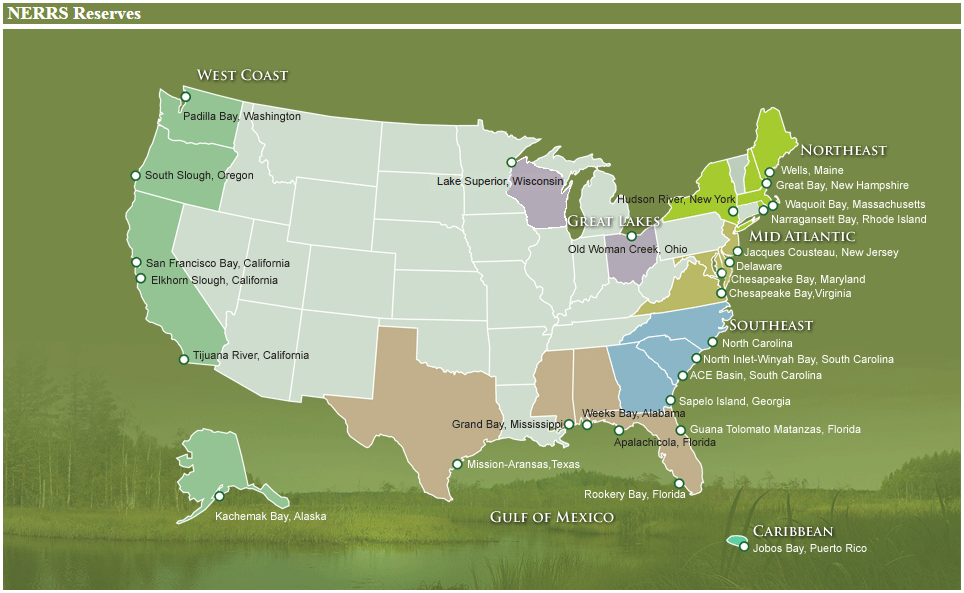
\includegraphics[width = 0.8\textwidth]{fig/NERRS_locations.png}}
\tiny
\flushright
\href{http://nerrs.noaa.gov/ReservesMap.aspx}{http://nerrs.noaa.gov/ReservesMap.aspx}
\end{frame}

%%%%%%
\begin{frame}{\textbf{Case 2: Improving estimates of metabolism}}{\textbf{Application to Gulf Coast estuaries}}
Metabolism was estimated using observed and `detided' DO time series
\end{frame}

% %%%%%%
% \begin{frame}{\textbf{Case 3: Open-source science}}{\textbf{Analysis tools for water quality data}}
% \onslide<+->
% The SWMP database and others like it represent incredible opportunities to further our knowledge of natural systems...\\~\\
% ...including the effects of eutrophication \\~\\
% \onslide<+->
% \alert{Problem:} These data are numerous and not easily compared\\~\\
% \alert{Solution:} Develop open-source tools that address the challenges of large-scale comparative analyses with continuous monitoring data\\~\\
% \onslide<+->
% The benefits include:
% \begin{itemize}
% \item Free for use by anyone
% \item Free to collaborate
% \item Facilitation of analysis with `under-the-hood' functionality
% \end{itemize}
% \end{frame}
% 
% %%%%%%
% \begin{frame}{\textbf{Case 3: Open-source science}}{\textbf{Analysis tools for water quality data}}
% \alert{SWMPr} is a freely available package for use with R \\~\\
% Designed to facilitate the analysis of SWMP data by providing functions that...\\~\\
% \begin{itemize}
% \item \alert{Retrieve} SWMP data for any site and date combination \\~\\ 
% \item \alert{Organize} the data using standard pre-processing techniques \\~\\
% \item \alert{Analyze} the data using a suite of exploratory and graphical analysis tools \\~\\
% \end{itemize}
% \end{frame}
% 
% %%%%%%
% \begin{frame}{\textbf{Case 3: Open-source science}}{\textbf{Analysis tools for water quality data}}
% What we've done so far... estimates of ecosystem metabolism 
% <</metab, message = F, fig = T, fig.width = 9, fig.height = 5, family = 'serif', cache = T, echo = F>>=
% 
% # load(file='M:/wq_models/SWMP/raw/rproc/dat_nem.RData')
% # 
% # sum.fun <- function(x){
% # 
% #   Pg <- mean(x$Pg,na.rm=T)
% #   Rt <- mean(x$Rt,na.rm=T)
% #   data.frame(Pg,Rt)
% #   
% #   }
% #   
% # to.plo <- lapply(dat.nem, function(x){
% #   x$Date <- as.numeric(strftime(x$Date, '%Y'))
% #   tmp <- lapply(split(x, x$Date), sum.fun)
% #   tmp <- do.call('rbind', tmp)
% #   sum.fun(tmp)
% #   })
% # nem_sum <- melt(to.plo)
% # save(nem_sum, file = 'data/nem_sum.RData')
% 
% load(file='data/nem_sum.RData')
% to.plo <- nem_sum
% 
% #reassign factors for ranking in plot
% sort.val<-order(to.plo[to.plo$variable=='Pg','value'])
% to.plo$L1<-factor(to.plo$L1)
% to.plo$L1<-factor(
%   to.plo$L1,
%   levels=levels(to.plo$L1)[sort.val],
%   labels=levels(to.plo$L1)[sort.val]
%   )
% new.labs<-c('Mean annual production','Mean annual respiration')
% to.plo$variable<-factor(to.plo$variable,levels=c('Pg', 'Rt'),labels=new.labs)
% 
% ylabs<-expression(paste('mmol ', O[2],' ', m^-2,' ', d^-1))
% 
% p<-ggplot(to.plo,aes(x=L1,y=value,group=variable,fill=variable)) + 
%   geom_bar(stat='identity') + 
%   scale_y_continuous(ylabs) + 
%   facet_wrap(~variable,ncol=1, scales = 'free_y') + 
%   scale_x_discrete(name=element_blank()) + 
%   theme_mine() + 
%   theme(
%     axis.text.x = element_text(angle = 90, vjust=0.5,hjust=1,size=6),
%     legend.position='none'
%     ) +
%   scale_fill_manual(values = pal(5)[c(2, 4)])
% print(p)
% @
% \end{frame}
% 
% %%%%%%
% \begin{frame}{\textbf{Case 3: Open-source science}}{\textbf{Analysis tools for water quality data}}
% \vspace{-0.1in}
% <<dtd_met, results = 'hold', cache = T, fig.height = 5.5, fig.width = 9, out.width = '\\textwidth', eval = T, echo = F, family = 'serif'>>=
% load('data/SAPDC_wtreg_12.RData')
% to_plo <- get('SAPDC_wtreg_12')
% 
% load('data/sapdc_met.RData')
% met_plo <- melt(sapdc_met, id.var = 'Date', measure.var = c('Pg', 'Rt', 'Pg_dtd', 'Rt_dtd'))
% met_plo$type <- rep('Observed', length = nrow(met_plo))
% met_plo$type[grep('dtd$', met_plo$variable)] <- 'Detided'
% met_plo$variable <- gsub('_dtd$', '', met_plo$variable)
% met_plo$type<- factor(met_plo$type, levels = c('Observed', 'Detided'), labels = c('Observed', 'Detided'))
% met_plo$variable <- factor(met_plo$variable, levels = c('Pg', 'Rt'), labels = c('Production', 'Respiration'))
% 
% ylab<-expression(paste('DO (mg ',L^-1,')'))
% p1 <- ggplot(to_plo, aes(x = DateTimeStamp)) + 
%   geom_line(aes(y = DO_obs, colour = 'Observed')) +
%   geom_line(aes(y = DO_nrm, colour = 'Detided')) +
%   scale_colour_manual('', values=pal(5)[c(2, 5)]) +
%   scale_y_continuous(ylab) +
%   theme_mine() +
%   theme(legend.position = 'top', axis.title.x = element_blank())
% 
% ylab<-expression(paste('mmol ', O[2],' ', m^-2,' ', d^-1))
% p2 <- ggplot(met_plo, aes(x = Date, y = value, group = variable, colour = variable)) + 
%   geom_line() +
%   geom_point() +
%   facet_wrap(~type, ncol = 1) + 
%   scale_colour_manual('', values=pal(5)[c(1, 3)]) +
%   scale_y_continuous(ylab) +
%   theme_mine() +
%   theme(legend.position = 'top', axis.title.x = element_blank())
% 
% grid.arrange(p1, p2, ncol = 1, heights = c(1.5,2))
% @
% \end{frame}
% 
% %%%%%%
% \begin{frame}{\textbf{Case 3: Open-source science}}{\textbf{Analysis tools for water quality data}}
% \onslide<+->
% Tools in the SWMPr package (or that will be included) have facilitated comparative analyses of millions of water quality records from NERRS \\~\\
% These tools can help improve our understanding of nutrient pollution and eutrophication \\~\\
% \onslide<+->
% Potential for many other applications... actively being developed \\~\\
% \begin{columns}
% \begin{column}{0.25\textwidth}
% \centerline{\includegraphics[width = \textwidth]{fig/Rlogo.png}}
% \end{column}
% \begin{column}{0.25\textwidth}
% \centerline{\includegraphics[width = \textwidth]{fig/RStudio.png}}
% \end{column}
% \begin{column}{0.25\textwidth}
% \centerline{\includegraphics[width = \textwidth]{fig/knit-logo.png}}
% \end{column}
% \begin{column}{0.25\textwidth}
% \centerline{\includegraphics[width = \textwidth]{fig/octocat.png}}
% \end{column}
% \end{columns}
% \end{frame}
% 
% \section{Conclusions}
% %%%%%%
% \begin{frame}{\textbf{Conclusions}}
% The analysis of water quality will continue to require the use of novel tecniques to interpret the data \\~\\
% These needs are motivated by: \\~\\
% \begin{itemize}
% \item The continued relevance of stressors that influence ecosystem conditions \\~\\
% \item Our increasing ability to gather raw, uninterpreted data \\~\\
% \end{itemize}
% Our methods must be able to make sense of \alert{historical trends}, as well as predict \alert{future conditions}
% \end{frame}
% 
% %%%%%%
% \begin{frame}{\textbf{Conclusions}}
% Our ability to \alert{share}, \alert{reproduce}, and \alert{collaborate} is essential \\~\\
% \alert{SWMPr package:} \href{https://github.com/fawda123/SWMPr}{https://github.com/fawda123/SWMPr} \\~\\
% \alert{Seagrass applications:} \href{https://beckmw.shinyapps.io/sg_depth}{https://beckmw.shinyapps.io/sg\_depth} \\~\\
% \alert{Ecosystem metabolism and detiding:} \href{http://spark.rstudio.com/beckmw/detiding_cases/}{http://spark.rstudio.com/beckmw/detiding\_cases/} \\~\\
% \alert{This presentation:} \href{https://github.com/fawda123/wqtrends_pres}{https://github.com/fawda123/wqtrends\_pres}
% \end{frame}
% 
% %%%%%%
% \begin{frame}
% Acknowledgments:\\~\\
% \begin{columns}
% \begin{column}{0.6\textwidth}
% {\footnotesize
% Research staff and employees at USEPA Gulf Ecology Division - especially J. Hagy, M. Murrell\\~\\
% Field staff and data managers at Hillsborough County Environmental Protection Commission\\~\\
% Research coordinators, technicians, and field staff of the National Estuarine Research Reserve System}\\~\\
% \end{column}
% \begin{column}{0.3\textwidth}
% \vspace{-0.2in}
% \begin{center}
% {\tiny
% Wes Anderson Zissou color theme borrowed and adapted from \href{https://github.com/karthik/wesanderson}{github.com/karthik}\\~\\
% \includegraphics[width=0.55\linewidth]{fig/zissou.png}\\~\\
% \vspace{-0.15in}
% \scalebox{0.7}{\hbox{\tiny Image credit:\thinspace{\tiny \href{http://stephenmorrow.deviantart.com/}{Stephen Morrow}}}}}
% \end{center}
% \end{column}
% \end{columns}
% \vfill
% Funding sources and contact:\\~\\
% \begin{columns}
% \begin{column}{0.5\textwidth}
% \centerline{
\includegraphics[width=0.4\linewidth]{fig/epa_logo.png}}
% \end{column}
% \begin{column}{0.5\textwidth}
% \scriptsize
% \href{mailto:beck.marcus@epa.gov}{beck.marcus@epa.gov} \\~\\
% Phone: 8509342480 \\~\\
% Github: \href{https://github.com/fawda123/}{github.com/fawda123/} \\~\\
% Blog: \href{http://beckmw.wordpress.com/}{beckmw.wordpress.com/}
% \end{column}
% \end{columns}
% \vspace{0.2in}
% \end{frame}

%%%%%%
\section{References}
\begin{frame}[allowframebreaks,t]{\textbf{References}}
\tiny
\setbeamertemplate{bibliography item}{}
\bibliographystyle{apalike_mine}
\bibliography{ref_diss}
\end{frame}

\end{document}
